\documentclass[../dissertation.tex]{subfiles}
\begin{document}

\chapter{Research}

\section{Background}

Initially, research done covered both network visualisation and specifically massive network visualisation, and as well as that, it looked into software that existed which visualised networks. In regards to the visualisation of massive networks, some important techniques learnt were:

\begin{itemize}
    \item Node grouping/bundling: This is when software uses algorithms to decide (with or without some form of user input) which nodes are very similar to each other, and upon establishing this relationship, groups them in to one node, generally visually different in some way (often by size or colour). This allows for hundreds or thousands of nodes to be grouped into one node and hence take up for less memory, processing power, bandwidth and screen space on the clients machine. A way to make this even more helpful is to show how the nodes being bundled interact with themselves, for example if they are heavily connected or all connected to just a few nodes, or if they are in a ring formation.
    \item Edge bundling: This is similar to node grouping but applied to edges, when several edges take very similar paths from one node (or group of nodes) to another, then the edges can be bundled into one edge. If node grouping is done then this process will have less of an impact as all of the edges will already be bundled together assuming the node grouping algorithm was successful. Like node bundling, it is often shown through the change of the size of the edge or the colour. See Figure \ref{fig:bundling}.
    \begin{figure}
        \centering
        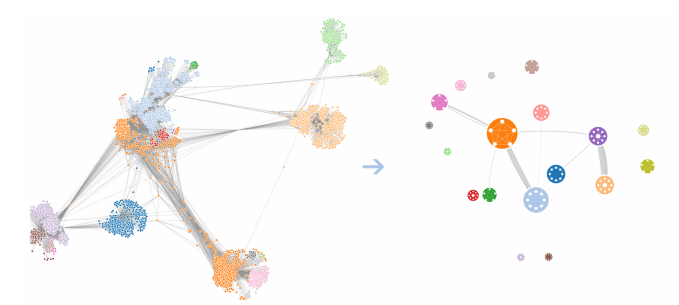
\includegraphics[width=15cm]{4/bundling}
        \caption{Demonstrates both node and edge bundling, where thickness of edge displays how many edges there are, and size of node indicates number of nodes group. On top of that, each node displays how nodes within it were connected together.}
        \label{fig:bundling}
    \end{figure}

    \item Local Edge Lens: This involves rendering all or part of the graph, and upon focusing on a section of the graph, that part is zoomed in or clarified as if through a lens and that part of the graph is zoomed in, becoming more clear. Another way of implementing this can be that when the lens is applied, it can render more information that was not shown before in order to save computational power. See Figure \ref{fig:local}.
    \begin{figure}
        \centering
        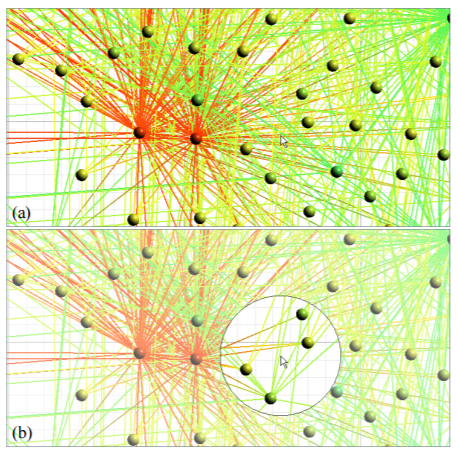
\includegraphics[width=8cm]{4/local}
        \caption{If a network is cluttered (a), then it can be hard to get useful information from it. A local edge lens (b) lets users easily identify which edges are connected to which nodes.}
        \label{fig:local}
    \end{figure}
    \item Deleting unnecessary content "smartly": This involves using an algorithm to remove certain nodes or edges that are deemed to be adding little or no useful information for the user. This algorithm can take no parameters, or work off a user's input, in which they specify what they are interested in, so other information is partially or fully removed. See Figure \ref{fig:deletion}.
    \begin{figure}
        \centering
        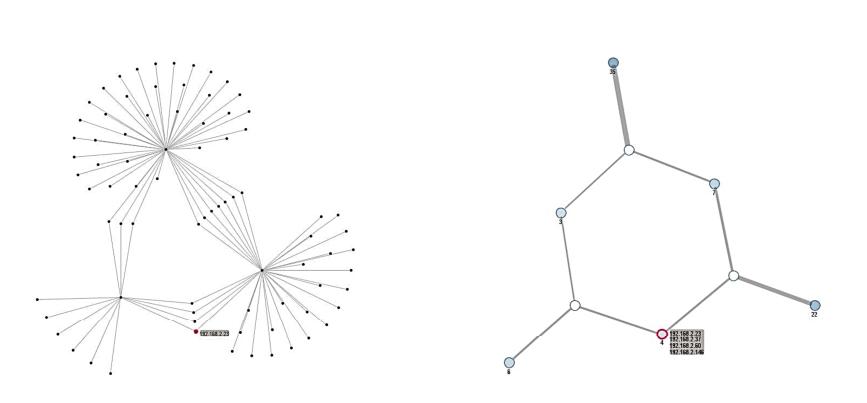
\includegraphics[width=15cm]{4/deletion}
        \caption{This figure clearly shoes how the deletion of many nodes does not always mean information is lost, and in some cases, information can become more clear as a result of the operation.}
        \label{fig:deletion}
    \end{figure}
\end{itemize}

\section{Current Graphing Software}

On top of finding out techniques used by software for large network visualisation, a list was also created of all software that was mentioned in papers or found during research that was related to large network visualisation. Quite often, the software mentioned had been hand-made for that project and was not feature complete, or the software could only be used for a price, but the below list contains the names of software that was reasonable to look further into, found by searching online and through mentions from papers:
\begin{itemize}
    \item GUESS
    \item SNAP
    \item Gephi
    \item GraphViz
    \item Tulip
    \item D3.js
    \item Vis.js
\end{itemize}

This software is reviewed below.

\section{Systematic Review of Existing Software}

\subsection{Aim} 

The goal of the research was to look into several different types of graphing software, and as a result, find out more about how network visualisation software. The software would be analysed for several characteristics, both related to general graphing of networks, and graphing of specifically huge networks.

\subsection{Methodology}

Upon finishing background research and defining a clear aim for the research, the next step was to come up with a list of criteria that each of the pieces of software would be compared against, and a robust process for how the software would be tested against the criteria. The process and criteria would ideally be based off an established way to systematically evaluate information visualisation. However, even after a long time was spent trying to find papers on that subject, it turned out to be surprisingly difficult to find out about testing software as a developer. Nearly all of the results found were about evaluating a system you had made and tended to be focused on getting professional testers to use the application or trialing the software on potential future end-users, as opposed to systematically evaluating systems.

The initial plan was to split the criteria into several categories and weigh each category as to its importance. 

The first criteria to assess would be how easy it is to get a basic network (5 or 10 nodes) displayed from scratch, from downloading the software and installing it, to understanding it's documentation, to getting a network displayed. 

After that, some more important criteria were how easy it is to load in a network from a file, and also, if the network was modified in any way between loading it in and displaying it to the used, or even while the user was viewing it, then saving the network to a file. 

The next features to be analysed for will be based on interactivity - how easily a user can edit the network to get more useful information out of it. This would include the ability to zoom into a part of the network or being able to pan or scroll. A more complex feature (that would be rarely used but would occasionally add valuable information to the user) would be the ability to make it dynamic - showing the change in a graph over time (or another parameter). 

A major criteria would then be how well the software would scale up to massive networks - this would include running tests on increasingly large networks and seeing how long the software takes, and also if it includes node or edge bundling or other ways of increasing clarity of massive networks. Time taken to render is also an important statistic, but less important than clarity for massive amounts of data for this project. This is perhaps the most important category as no matter the above features, if the network is not clear for huge numbers of nodes / edges then it does not answer the problem at hand. A feature that would be desired to increase user clarity would be the ability to view the network in many different layouts - which would give users more flexibility and would often lead to better understanding. 

This set of criteria was compiled into a list which was to act as the process for the experiment. 

\begin{enumerate}
	\item Standalone or library
	\item Documentation:
	\begin{enumerate}
		\item Is it easy to understand - explained clearly and concisely?
		\item Is it Comprehensive - software fully documented?
		\item Length of time until confident beginning to use system?
	\end{enumerate}
	\item Time until a simple hard-coded graph could be displayed?
	\item Can a file be loaded into the system?
	\item Can a network be exported to a file?
	\item How long it took to render the graph of:
	\begin{enumerate}
	    \item 30 nodes
	    \item 200 nodes
	    \item 1000 nodes
	    \item 3000 nodes
	\end{enumerate}
	\item If the software allowed for:
	\begin{enumerate}
		\item Zooming
		\item Panning
		\item Scrolling
	\end{enumerate}
	\item Can a graph be dynamic - allowing data taken at multiple points over time to be viewed?
	\item Does the software included features for displaying huge graphs:
	\begin{enumerate}
		\item Edge Bundling
		\item Node bundling
		\item Alternative layout options
	\end{enumerate}
	\item Can a graph be multivariate?
	\item Is there a possibility of changing graphical settings for the network?
	\item Can a graph be displayed in 3D?
	\item Any other idiosyncrasies?
\end{enumerate}

Each piece of software was to be evaluated against this criteria, with the goal of both finding out which pieces of software were more successful, over many parameters, and also to become more familiar with graphing software used in industry.

\subsection{Data and Results}

Upon beginning to run the experiment, it became clear that several pieces of software would not be able to be assessed by the criteria created previously, for a number of reasons.

\subsubsection{GUESS}

The first piece of software, GUESS, was software that never left beta, and was last developed in 2007. This meant that the software had fairly little documentation and what it did have was poor. On top of this, the wiki no longer existed which meant many of the links to documentation on the website were broken. Despite it looking promising, it became clear it would not be usable.

\subsubsection{SNAP}

This piece of software could not be compared to much of the criteria as the purpose of it is to analyse and manipulate graphs, as opposed to also visualise them. However, time was spent reading it’s documentation and going through all the sample code snippets to understanding how the software worked to some degree. The reason this was done was that it both felt important to have some knowledge of how network manipulation software worked, and also depending on the direction the project took, network manipulation may well be used in order to bundle edges or nodes in order to increase performance of massive networks.

Due to the above limitation, at this point GUESS and SNAP were considered no longer appropriate. This left the remaining five software packages to be analysed and compared to the research criteria, stated above.

\subsubsection{Gephi}

This was the first software package that was as expected, and was fairly easy to test, use and was well documented. After about half an hour I was comfortable with how it worked, able to make simple graphs, and to import graphs from many formats (CSV, GDF, QML, GraphML, net, etc.) and export to all of them, along with as a PNG, PDF or SVG. It supported zooming, panning and scrolling, and having data being dynamic was a possibility. There was also multiple heavily customisable layout options, some of which would suit large networks more than others, although there was no additional support for large networks, other than the system being very efficient (bundling was not supported, along with partial viewing of the data). Additionally, there was the ability to change graphical settings, have the data graphed in 3D, and have a multivariate graph.

\subsubsection{Graphviz}

Graphviz was difficult to test, being a collection of software as opposed to a single package. Most of the packages were not fit for purpose, often displaying data in charts, for example. The package I ended up testing was 'sfdp'. Although it fitted most of the criteria and claimed to support large networks, it turned out to be very focused on graphing far smaller networks with little support for anything of a few thousand nodes or more. The documentation was okay, and the software had the ability to import and export as a very large amount of file formats. It also supported zooming/panning/scrolling, but the UI clearly was not build around supporting large networks, with information becoming very unclear quickly. There was also no explicit support for visualising massive networks.

\url{http://www.graphviz.org/content/root} - this shows how the UI is clearly focused towards smaller networks of up to a thousand nodes or so.

\subsubsection{Tulip}

Tulip is an information visualisation framework that also lets you both visualise and analyse the data. It is very easy to use and is well documented, allows for easy importing and exporting of networks, and is really fast, allowing for 3000 nodes to be visualised instantly. 

It is worth noting that on the university lab machines, without admin access, it was not possible to install Tulip, which meant I ended up installing it on Windows (the computer that Tulip was ran on is far more powerful than the university machines and there is a very reasonable chance that on the lab machines Tulip would not perform as well). However, it seemed very good quality software. It also included edge bundling and 'clustering' (a type of node bundling).

\subsubsection{D3.js}

D3.js is a JavaScript library for data visualisation. The library is far more flexible than the rest of the software tested, but requires far more setup to be done by the user. The documentation is good although it is more complicated that other most of the other programs, and importing and exporting is easily possible via JSON, and other file formats with slightly greater difficulty. It supports zooming / panning / scrolling as expected. Also, there are many ways to make it effective at showing massive networks, but this would require research into many different packages and potentially writing a lot code to do it.

\subsubsection{Vis.js}

Vis.js is, like D3.js, a JavaScript library for data visualisation. However, unlike D3.js, it is not hugely flexible but much easier to get a basic network setup. The documentation is very good and importing and exporting is easily possible via JSON. It also includes some node bundling options which could be looked into at a future date.

\subsubsection{Comparisons}

For the majority of the criteria, all of the software packages performed very similarly. 
\\
TODO: Insert (more) tables and remove (more) data from above where appropriate.
\\
TODO: Something like "all of the above supported scrolling/zooming/panning."

See Table \ref{table:render-times} for render times.

\begin{table}[h]
\centering
\label{table:render-times}
\begin{tabular}{|l|l|l|l|l|}
    \hline
             & 30      & 200     & 1000    & 3000    \\
    \hline
    Gephi    & Instant & Instant & Instant & 0.5     \\
    \hline
    Graphviz & Instant & 0.3     & 1       & 3       \\
    \hline
    Tulip    & Instant & Instant & Instant & Instant \\
    \hline
    D3.js    & todo    & todo    & todo    & todo    \\
    \hline
    Vis.js   & todo    & todo    & todo    & todo   \\
    \hline
\end{tabular}
\caption{This shows how long it took each of the different pieces of software to render the specified number of nodes}
\end{table}


\subsection{Conclusion}

Following the process outlined above was difficult as software APIs were expected which could be easily compared by minor differences, but most of the software were standalone packages and were more difficult to compare. Also, none of the software would be directly suitable for SAS apart from the JavaScript libraries as the other pieces of software were standalone applications as opposed to libraries that could be utilised by a web application. Considering that the results were difficult to both gain and easily differentiate, this highlighted the complexities comparing such diverse software, as well as the lack of software suitable to compare against the criteria.

However, given all of the above data and comparisons, Tulip was chosen as the most fitting software, performing the best under both light and heavy load, and also having a very fully-featured API in both C++ and Python (a C++ wrapper).

\section{Next Steps}

As a result of the outcome of research, there were several different directions that the project could go:

\begin{itemize}
    \item Write several different programs in JavaScript (or Python etc.) that alter huge graphs by bundling etc. and compare how they become easier to visualise and/or render using D3.js This would include using several large networks of different types (sparse or very interconnected) and use different algorithms or techniques to see what is the most efficient way or best way to evaluate.
    \item Evaluate several different types of graphing software (Tulip/Gephi/GraphViz) and see where they begin to fail and what their bottlenecks are. 
    \item Look into database systems that visualise data too. Many database packages allow for data visualisation.
    \item Build a web application for one of the pieces of desktop software in order to allow users to access a system and visualise a huge amount of data without the need for an extremely powerful machine.
\end{itemize} 

After much discussion and thought, it was decided that a web application would be built for the project, based on the Tulip Python API. This would result in a users being able to access a wealth of information without owning a huge amount of computational power, which could benefit both employees of a business, allowing them to work from home on less powerful devices and without the need for huge data connections, and also clients of a business, needing lower specification machines, which leads to more possible clients for a business.

\end{document}